% Options for packages loaded elsewhere
\PassOptionsToPackage{unicode}{hyperref}
\PassOptionsToPackage{hyphens}{url}
%
\documentclass[
]{article}
\usepackage{amsmath,amssymb}
\usepackage{lmodern}
\usepackage{iftex}
\ifPDFTeX
  \usepackage[T1]{fontenc}
  \usepackage[utf8]{inputenc}
  \usepackage{textcomp} % provide euro and other symbols
\else % if luatex or xetex
  \usepackage{unicode-math}
  \defaultfontfeatures{Scale=MatchLowercase}
  \defaultfontfeatures[\rmfamily]{Ligatures=TeX,Scale=1}
\fi
% Use upquote if available, for straight quotes in verbatim environments
\IfFileExists{upquote.sty}{\usepackage{upquote}}{}
\IfFileExists{microtype.sty}{% use microtype if available
  \usepackage[]{microtype}
  \UseMicrotypeSet[protrusion]{basicmath} % disable protrusion for tt fonts
}{}
\makeatletter
\@ifundefined{KOMAClassName}{% if non-KOMA class
  \IfFileExists{parskip.sty}{%
    \usepackage{parskip}
  }{% else
    \setlength{\parindent}{0pt}
    \setlength{\parskip}{6pt plus 2pt minus 1pt}}
}{% if KOMA class
  \KOMAoptions{parskip=half}}
\makeatother
\usepackage{xcolor}
\IfFileExists{xurl.sty}{\usepackage{xurl}}{} % add URL line breaks if available
\IfFileExists{bookmark.sty}{\usepackage{bookmark}}{\usepackage{hyperref}}
\hypersetup{
  pdftitle={Homework 3: Propensity Score Matching Analysis},
  pdfauthor={Xuange Liang},
  hidelinks,
  pdfcreator={LaTeX via pandoc}}
\urlstyle{same} % disable monospaced font for URLs
\usepackage{longtable,booktabs,array}
\usepackage{calc} % for calculating minipage widths
% Correct order of tables after \paragraph or \subparagraph
\usepackage{etoolbox}
\makeatletter
\patchcmd\longtable{\par}{\if@noskipsec\mbox{}\fi\par}{}{}
\makeatother
% Allow footnotes in longtable head/foot
\IfFileExists{footnotehyper.sty}{\usepackage{footnotehyper}}{\usepackage{footnote}}
\makesavenoteenv{longtable}
\setlength{\emergencystretch}{3em} % prevent overfull lines
\providecommand{\tightlist}{%
  \setlength{\itemsep}{0pt}\setlength{\parskip}{0pt}}
\setcounter{secnumdepth}{5}
% Shared LaTeX style for homework submissions
\usepackage{microtype}
\usepackage{booktabs}
\usepackage{longtable}
\usepackage{array}
\usepackage{caption}
\usepackage{fancyhdr}
\usepackage{titlesec}
\usepackage{setspace}
\usepackage{float}
\usepackage{graphicx}
\usepackage[table]{xcolor}
\usepackage{enumitem}
\usepackage[most]{tcolorbox}
\usepackage{geometry}

% Wider margins to accommodate tables
\geometry{left=2.2cm, right=2.2cm, top=2.5cm, bottom=2.5cm}

\definecolor{TitleBlue}{HTML}{0B3C5D}
\definecolor{SoftGray}{HTML}{F6F8FA}

\setstretch{1.15}
\setlength{\parskip}{4pt}
\setlength{\parindent}{0pt}

% Use small font in all longtable environments to prevent overflow
\AtBeginEnvironment{longtable}{\small}

\titleformat{\section}{\large\bfseries\color{TitleBlue}}{\thesection}{0.6em}{}
\titleformat{\subsection}{\normalsize\bfseries\color{TitleBlue}}{\thesubsection}{0.6em}{}

\captionsetup{
  font=small,
  labelfont=bf
}

\rowcolors{2}{SoftGray}{white}
\setlist[itemize]{leftmargin=*, topsep=2pt, itemsep=1pt}
\setlist[enumerate]{leftmargin=*, topsep=2pt, itemsep=1pt}

\pagestyle{fancy}
\fancyhf{}
\fancyhead[L]{\small\nouppercase{\leftmark}}
\fancyhead[R]{\small P8586 Applied Methods}
\fancyfoot[C]{\thepage}
\setlength{\headheight}{15pt}
\addtolength{\topmargin}{-1pt}
% Prevent header text overflow by limiting left header width
\renewcommand{\headrulewidth}{0.4pt}

\AtBeginDocument{
  \hypersetup{
    colorlinks=true,
    linkcolor=TitleBlue,
    urlcolor=TitleBlue,
    citecolor=TitleBlue
  }
}

% Keep title and TOC on same page, content starts on new page
\AtBeginDocument{
  \let\oldtableofcontents\tableofcontents
  \renewcommand{\tableofcontents}{%
    \oldtableofcontents
    \clearpage
  }
}
\ifLuaTeX
  \usepackage{selnolig}  % disable illegal ligatures
\fi

\title{Homework 3: Propensity Score Matching Analysis}
\author{Xuange Liang}
\date{February 24, 2026}

\begin{document}
\maketitle

{
\setcounter{tocdepth}{3}
\tableofcontents
}
% \hypertarget{introduction}{%
% \section{Introduction}\label{introduction}}

% This analysis applies propensity score (PS) matching to examine the
% causal association between intraventricular hemorrhage (IVH) and
% mortality among very low birth weight (VLBW) infants. The cohort
% consists of 514 infants with birth weight \textless{} 1,600 g born at
% Duke University Medical Center between 1981 and 1987. The exposure of
% interest is IVH (ivh2 = 1, present in 84 infants; 16.3\%), and the
% primary outcome is in-hospital death (dead = 1). Measured potential
% confounders include birth weight, gestational age, pneumothorax, mode of
% delivery, multiple gestation, and birth location.

% Propensity score matching creates a pseudo-randomized comparison group
% by balancing baseline covariates between IVH-exposed and unexposed
% infants, providing a more rigorous estimate of the causal effect than
% conventional multivariable adjustment alone.

\begin{center}\rule{0.5\linewidth}{0.5pt}\end{center}

\hypertarget{requirement-1-ps-step-1-model-model-selection}{%
\section{Requirement 1: PS Step 1 Model --- Model
Selection}\label{requirement-1-ps-step-1-model-model-selection}}

\hypertarget{model-specification}{%
\subsection{Model Specification}\label{model-specification}}

The propensity score is defined as the conditional probability of having
IVH given baseline covariates: pneumothorax (pneumo), multiple gestation
(twin), mode of delivery (Delivery\_new), birth location (Inout\_new),
birth weight category (bwt\_cat), and gestational age category
(gest\_cat). Two logistic regression models were fitted:

\begin{itemize}
\tightlist
\item
  \textbf{Model A (No Interactions):} Main effects only.
\item
  \textbf{Model B (Two-Way Interactions, Backward):} All two-way
  interaction terms, backward stepwise at SLS = 0.20.
\end{itemize}

\hypertarget{roc-curves}{%
\subsection{ROC Curves}\label{roc-curves}}

\begin{figure}[H]
\centering
\begin{minipage}[t]{0.48\textwidth}
\centering
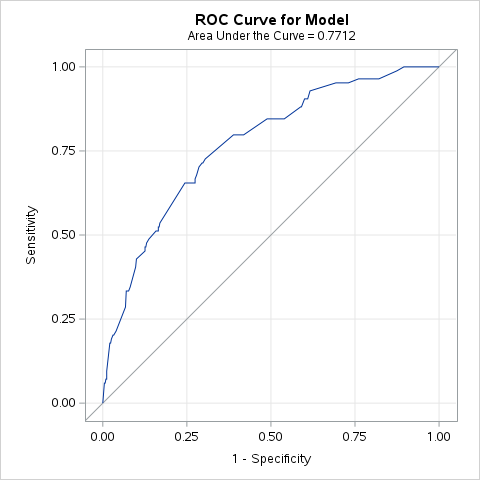
\includegraphics[width=\linewidth]{fig_roc_modelA.png}
\caption*{\textbf{Model A: No Interaction Terms}\\C-statistic = 0.771\\N of matched cohort = 164 (82 pairs)\\Hosmer-Lemeshow p-value $\geq$ 0.05\\Quasi-complete separation: No}
\end{minipage}
\hfill
\begin{minipage}[t]{0.48\textwidth}
\centering
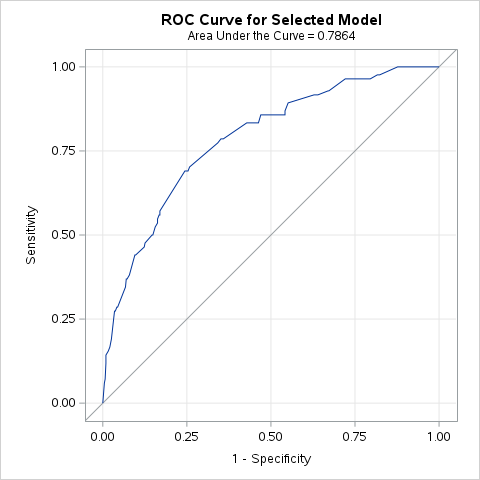
\includegraphics[width=\linewidth]{fig_roc_modelB.png}
\caption*{\textbf{Model B: Two-Way Interactions (Backward, SLS=0.20)}\\C-statistic = 0.786\\N of matched cohort = 164 (82 pairs)\\Hosmer-Lemeshow: not available (selection model)\\\textbf{WARNING: Quasi-complete separation detected}}
\end{minipage}
\end{figure}

\hypertarget{model-comparison-and-final-model-selection}{%
\subsection{Model Comparison and Final Model
Selection}\label{model-comparison-and-final-model-selection}}

\begin{longtable}[]{@{}lcc@{}}
\toprule
Criterion & Model A (No Interactions) & Model B (Interactions,
Backward) \\
\midrule
\endhead
C-statistic (AUC) & 0.771 & 0.786 \\
Hosmer-Lemeshow p-value & \(\geq\) 0.05 (good fit) & Not available \\
Quasi-complete separation & No & \textbf{Yes (warning issued)} \\
Matched cohort size & 164 (82 pairs) & 164 (82 pairs) \\
Max SMD after matching (binary vars) & 0.151 & 0.151 \\
\bottomrule
\end{longtable}

The following table shows the standardized mean differences (SMD) for
each covariate in the matched cohort under Model A:

\begin{longtable}[]{@{}clc@{}}
\toprule
Obs & Variable & Std Difference (Model A Matched) \\
\midrule
\endhead
1 & Logit Propensity Score & 0.0105 \\
2 & pneumo\_yes & -0.0558 \\
3 & twin\_yes & 0.0342 \\
4 & delivery\_vag & 0.0000 \\
5 & inout\_transport & 0.0578 \\
6 & bwt\_lt1000 & -0.1252 \\
7 & bwt\_1000\_1299 & 0.1512 \\
8 & gest\_lt28 & -0.0259 \\
9 & gest\_28\_31 & 0.0492 \\
\bottomrule
\end{longtable}

\textbf{Decision: Model A (no interactions) was selected as the final
propensity score model.} Although Model B has a marginally higher AUC
(0.786 vs.~0.771), it produced quasi-complete separation warnings due to
small cell sizes in interaction terms relative to the limited sample
size (N = 514), indicating numerical instability. Both models produced
the same matched cohort size and equivalent balance (all SMD \textless{}
0.2). For small samples, balance is considered acceptable if SMD
\textless{} 0.2; Model A satisfies this criterion for all covariates
with greater numerical stability.

\hypertarget{final-model-a-parameter-estimates}{%
\subsection{Final Model A: Parameter
Estimates}\label{final-model-a-parameter-estimates}}

\begin{longtable}[]{@{}llcccc@{}}
\toprule
Covariate & Level & Estimate & OR & 95\% CI & p-value \\
\midrule
\endhead
Intercept & & -4.4905 & --- & --- & \textless{} 0.001 \\
Pneumothorax & Yes vs.~No & 1.3116 & 3.712 & (2.073, 6.648) &
\textless{} 0.001 \\
Multiple Gestation & Yes vs.~No & -1.1410 & 0.319 & (0.136, 0.751) &
0.009 \\
Mode of Delivery & Vaginal vs.~C-Section & 0.7784 & 2.178 & (1.234,
3.844) & 0.007 \\
Birth Location & Transport vs.~Duke & 0.9445 & 2.571 & (1.458, 4.535) &
0.001 \\
Birth Weight & \textless{} 1000g vs.~\(\geq\) 1300g & 0.6698 & 1.954 &
(0.785, 4.861) & 0.150 \\
Birth Weight & 1000--1299g vs.~\(\geq\) 1300g & 0.4472 & 1.564 & (0.711,
3.440) & 0.266 \\
Gestational Age & \textless{} 28 wks vs.~\(\geq\) 32 wks & 1.6278 &
5.093 & (1.028, 25.221) & 0.046 \\
Gestational Age & 28--31 wks vs.~\(\geq\) 32 wks & 1.6220 & 5.063 &
(1.145, 22.400) & 0.033 \\
\bottomrule
\end{longtable}

\emph{C-statistic = 0.771. Pneumothorax, birth location, gestational
age, and mode of delivery were significant independent predictors of
IVH.}

\begin{center}\rule{0.5\linewidth}{0.5pt}\end{center}

\hypertarget{requirement-2-table-1-baseline-characteristics-before-and-after-matching}{%
\section{Requirement 2: Table 1 --- Baseline Characteristics Before and
After
Matching}\label{requirement-2-table-1-baseline-characteristics-before-and-after-matching}}

Greedy 1:1 nearest-neighbor matching was performed using PROC PSMATCH
with a caliper of 0.25 on the logit of the propensity score (Model A).
Of 514 infants in the original cohort (84 IVH-exposed; 430 unexposed),
\textbf{164 infants (82 per group) were successfully matched}, using
97.6\% of IVH-exposed infants.

\hypertarget{covariate-balance-love-plot}{%
\subsection{Covariate Balance --- Love
Plot}\label{covariate-balance-love-plot}}

\begin{figure}[H]
\centering
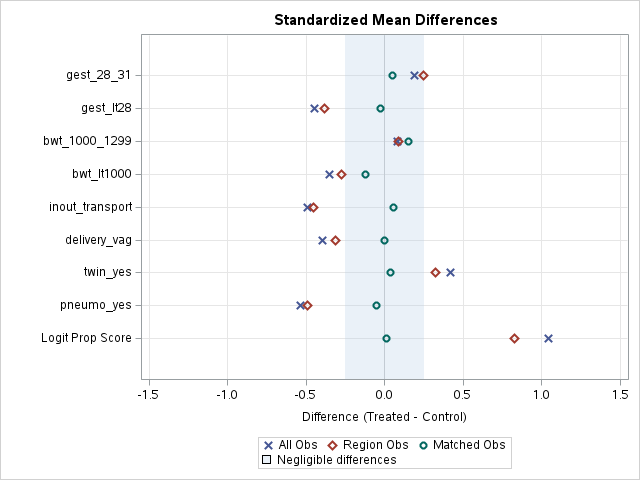
\includegraphics[width=0.85\textwidth]{fig_love_plot.png}
\caption*{\textbf{Figure 1: Standardized Difference Plot (Love Plot)}\\Standardized mean differences for all covariates before matching (blue/triangle) and after 1:1 PS matching (red/circle). All post-matching SMDs fall below the 0.2 threshold, confirming adequate covariate balance.}
\end{figure}

\hypertarget{table-1-baseline-characteristics-by-ivh-status-original-cohort-n-514}{%
\subsection{Table 1: Baseline Characteristics by IVH Status --- Original
Cohort (N =
514)}\label{table-1-baseline-characteristics-by-ivh-status-original-cohort-n-514}}

\begin{longtable}[]{@{}lcccc@{}}
\toprule
Covariate & No IVH (N = 430) & IVH (N = 84) & p-value & SMD \\
\midrule
\endhead
\textbf{Pneumothorax} & & & \textbf{\textless{} 0.001} & --- \\
 No & 357 (83.0\%) & 50 (59.5\%) & & \\
 Yes & 73 (17.0\%) & 34 (40.5\%) & & \\
\textbf{Multiple Gestation} & & & 0.002 & --- \\
 Singleton & 330 (76.7\%) & 77 (91.7\%) & & \\
 Multiple & 100 (23.3\%) & 7 (8.3\%) & & \\
\textbf{Mode of Delivery} & & & 0.001 & --- \\
 C-Section & 221 (51.4\%) & 27 (32.1\%) & & \\
 Vaginal & 209 (48.6\%) & 57 (67.9\%) & & \\
\textbf{Birth Location} & & & \textbf{\textless{} 0.001} & --- \\
 Born at Duke & 366 (85.1\%) & 54 (64.3\%) & & \\
 Transport & 64 (14.9\%) & 30 (35.7\%) & & \\
\textbf{Birth Weight Category} & & & 0.004 & --- \\
 \textless{} 1000 g & 146 (34.0\%) & 43 (51.2\%) & & \\
 1000--1299 g & 170 (39.5\%) & 30 (35.7\%) & & \\
 1300--1599 g & 114 (26.5\%) & 11 (13.1\%) & & \\
\textbf{Gestational Age Category} & & & \textbf{\textless{} 0.001} &
--- \\
 \textless{} 28 weeks & 114 (26.5\%) & 40 (47.6\%) & & \\
 28--31 weeks & 255 (59.3\%) & 42 (50.0\%) & & \\
 \(\geq\) 32 weeks & 61 (14.2\%) & 2 (2.4\%) & & \\
\bottomrule
\end{longtable}

\emph{Column percentages shown. Chi-square p-values. In the original
cohort, IVH-exposed infants differed significantly from unexposed
infants across all six covariates, confirming substantial baseline
confounding. IVH-exposed infants were more likely to have pneumothorax
(40.5\% vs.~17.0\%), be transported in (35.7\% vs.~14.9\%), have lower
gestational age (\textless{} 28 wks: 47.6\% vs.~26.5\%), and lower birth
weight (\textless{} 1000g: 51.2\% vs.~34.0\%).}

\begin{center}\rule{0.5\linewidth}{0.5pt}\end{center}

\hypertarget{table-1-baseline-characteristics-by-ivh-status-ps-matched-cohort-n-164}{%
\subsection{Table 1: Baseline Characteristics by IVH Status --- PS
Matched Cohort (N =
164)}\label{table-1-baseline-characteristics-by-ivh-status-ps-matched-cohort-n-164}}

\begin{longtable}[]{@{}lcccc@{}}
\toprule
Covariate & No IVH (N = 82) & IVH (N = 82) & p-value & SMD \\
\midrule
\endhead
\textbf{Pneumothorax} & & & 0.747 & -0.056 \\
 No & 52 (63.4\%) & 50 (61.0\%) & & \\
 Yes & 30 (36.6\%) & 32 (39.0\%) & & \\
\textbf{Multiple Gestation} & & & 0.787 & 0.034 \\
 Singleton & 74 (90.2\%) & 75 (91.5\%) & & \\
 Multiple & 8 (9.8\%) & 7 (8.5\%) & & \\
\textbf{Mode of Delivery} & & & 1.000 & 0.000 \\
 C-Section & 27 (32.9\%) & 27 (32.9\%) & & \\
 Vaginal & 55 (67.1\%) & 55 (67.1\%) & & \\
\textbf{Birth Location} & & & 0.744 & 0.058 \\
 Born at Duke & 52 (63.4\%) & 54 (65.9\%) & & \\
 Transport & 30 (36.6\%) & 28 (34.1\%) & & \\
\textbf{Birth Weight Category} & & & 0.629 & --- \\
 \textless{} 1000 g & 37 (45.1\%) & 42 (51.2\%) & & \\
 1000--1299 g & 35 (42.7\%) & 29 (35.4\%) & & \\
 1300--1599 g & 10 (12.2\%) & 11 (13.4\%) & & \\
\textbf{Gestational Age Category} & & & 0.821 & --- \\
 \textless{} 28 weeks & 38 (46.3\%) & 39 (47.6\%) & & \\
 28--31 weeks & 43 (52.4\%) & 41 (50.0\%) & & \\
 \(\geq\) 32 weeks & 1 (1.2\%) & 2 (2.4\%) & & \\
\bottomrule
\end{longtable}

\emph{Column percentages shown. After 1:1 PS matching, all p-values
exceed 0.62 and all SMDs are well below 0.2 (maximum binary-variable SMD
= 0.151 for bwt\_1000\_1299), indicating adequate covariate balance.}

\textbf{Plain-language interpretation of Table 1:} Before matching,
IVH-exposed infants were born earlier, weighed less, were more likely to
have pneumothorax, and were more frequently transported in from other
hospitals --- all characteristics reflecting the typical clinical
profile of severe prematurity. These imbalances mean any simple
comparison of death rates between IVH and non-IVH groups would conflate
the effect of IVH with the effect of being more premature. After
propensity score matching, both groups look essentially identical on all
measured characteristics (all p-values \textgreater{} 0.6), confirming
that the matched comparison is valid and free from the measured
confounders.

\begin{center}\rule{0.5\linewidth}{0.5pt}\end{center}

\hypertarget{requirement-3-propensity-score-distribution-before-and-after-matching}{%
\section{Requirement 3: Propensity Score Distribution Before and After
Matching}\label{requirement-3-propensity-score-distribution-before-and-after-matching}}

\hypertarget{ps-distribution-original-cohort-before-matching}{%
\subsection{PS Distribution --- Original Cohort (Before
Matching)}\label{ps-distribution-original-cohort-before-matching}}

\begin{figure}[H]
\centering
\begin{minipage}[t]{0.54\textwidth}
\centering
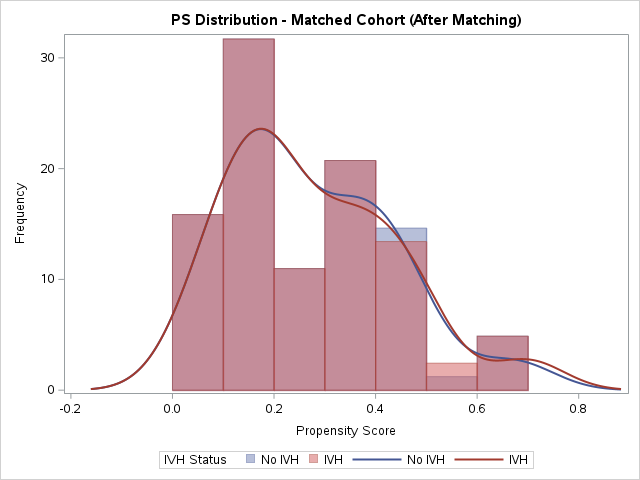
\includegraphics[width=\linewidth]{fig_ps_before_hist.png}
\end{minipage}
\hfill
\begin{minipage}[t]{0.43\textwidth}
\centering
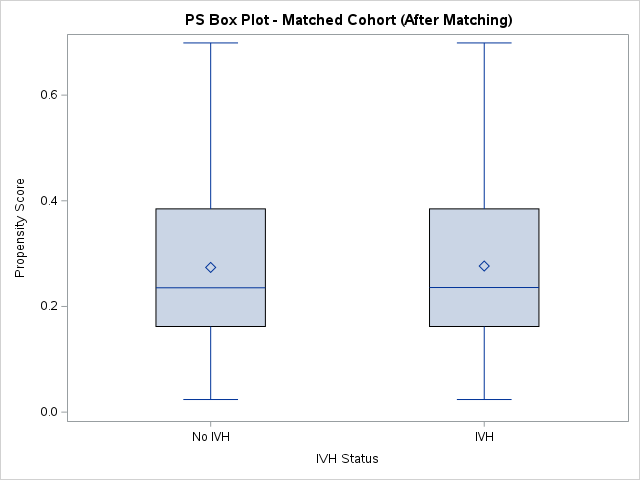
\includegraphics[width=\linewidth]{fig_ps_before_box.png}
\end{minipage}
\caption*{\textbf{Figure 2: PS Distribution — Original Cohort (N = 514)}\\Mean PS: IVH = 0.286, No IVH = 0.140. The two groups' PS distributions are clearly separated, reflecting substantial baseline imbalance before matching.}
\end{figure}

\hypertarget{ps-distribution-ps-matched-cohort-after-matching}{%
\subsection{PS Distribution --- PS Matched Cohort (After
Matching)}\label{ps-distribution-ps-matched-cohort-after-matching}}

\begin{figure}[H]
\centering
\begin{minipage}[t]{0.54\textwidth}
\centering
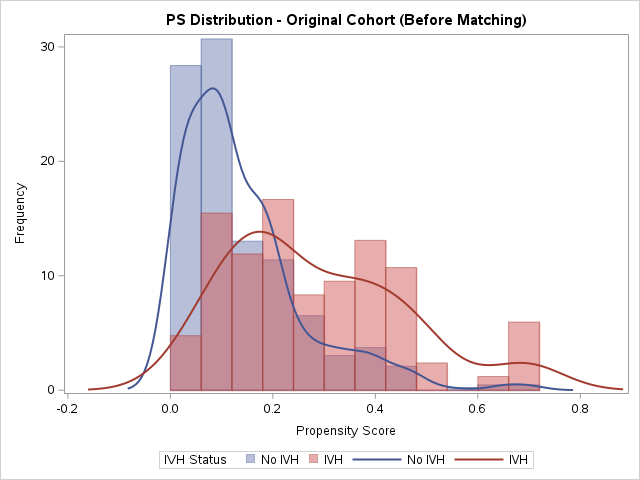
\includegraphics[width=\linewidth]{fig_ps_after_hist.png}
\end{minipage}
\hfill
\begin{minipage}[t]{0.43\textwidth}
\centering
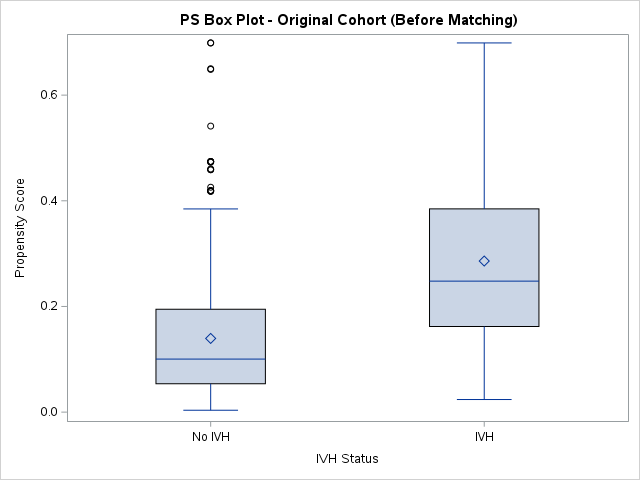
\includegraphics[width=\linewidth]{fig_ps_after_box.png}
\end{minipage}
\caption*{\textbf{Figure 3: PS Distribution — PS Matched Cohort (N = 164, 82 pairs)}\\Mean PS: IVH = 0.277, No IVH = 0.274. After matching, the two distributions are nearly identical, confirming successful balance within the region of common support.}
\end{figure}

\textbf{Plain-language interpretation:} Before matching, IVH-exposed
infants had much higher propensity scores (mean 0.286) than unexposed
infants (mean 0.140), reflecting their systematically higher baseline
risk driven by prematurity. The histograms show largely non-overlapping
distributions. After greedy 1:1 matching with a caliper of 0.25 on the
logit PS, both groups had nearly identical PS distributions (mean IVH =
0.277 vs.~No IVH = 0.274). The overlapping histograms and aligned box
plots confirm that matched controls were truly comparable to IVH-exposed
cases in terms of their predicted probability of having IVH.

\begin{center}\rule{0.5\linewidth}{0.5pt}\end{center}

\hypertarget{requirement-4-table-2-unadjusted-adjusted-and-ps-matched-estimates}{%
\section{Requirement 4: Table 2 --- Unadjusted, Adjusted, and PS-Matched
Estimates}\label{requirement-4-table-2-unadjusted-adjusted-and-ps-matched-estimates}}

Three approaches were used to estimate the association between IVH and
mortality:

\begin{enumerate}
\def\labelenumi{\arabic{enumi}.}
\tightlist
\item
  \textbf{Unadjusted:} Simple logistic regression (OR) and Poisson
  regression (RR) with IVH as the only predictor.
\item
  \textbf{Adjusted (HW1 Model):} Multivariable logistic and Poisson
  regression with IVH + pneumothorax + bwt\_cat + gest\_cat (purposeful
  selection from HW1).
\item
  \textbf{PS-Matched:} Conditional logistic regression stratified on
  matched pair ID (for OR); GEE Poisson regression with matched pair
  clustering (for RR).
\end{enumerate}

\hypertarget{table-2-ivh-and-mortality-distribution-and-effect-estimates}{%
\subsection{Table 2: IVH and Mortality --- Distribution and Effect
Estimates}\label{table-2-ivh-and-mortality-distribution-and-effect-estimates}}

\textbf{Mortality distribution by IVH status (row \%):}

\begin{longtable}[]{@{}lcc@{}}
\toprule
& Dead = 0 (Alive) & Dead = 1 (Dead) \\
\midrule
\endhead
\textbf{No IVH} (N = 430) & 372 (86.5\%) & 58 (13.5\%) \\
\textbf{IVH} (N = 84) & 43 (51.2\%) & 41 (48.8\%) \\
\bottomrule
\end{longtable}

\textbf{Association estimates (IVH vs.~No IVH):}

\begin{longtable}[]{@{}lcccc@{}}
\toprule
Method & OR (95\% CI) & p-value & RR (95\% CI) & p-value \\
\midrule
\endhead
Unadjusted & 6.116 (3.674, 10.179) & \textless{} 0.001 & 3.619 (2.426,
5.398) & \textless{} 0.001 \\
Adjusted (HW1) & 4.149 (2.291, 7.516) & \textless{} 0.001 & 2.059
(1.351, 3.137) & \textless{} 0.001 \\
PS-Matched & 3.857 (1.680, 8.857) & 0.002 & 2.053 (1.349, 3.124) &
\textless{} 0.001 \\
\bottomrule
\end{longtable}

Adjusted (HW1): multivariable model including pneumothorax, birth weight
category, and gestational age category. PS-Matched OR: conditional
logistic regression stratified on MatchID. PS-Matched RR: GEE Poisson
regression with MatchID as clustering unit.

\textbf{Plain-language interpretation of Table 2:}

\begin{itemize}
\item
  \textbf{Unadjusted:} IVH-exposed infants had 6.1 times the odds of
  dying (OR = 6.116) and 3.6 times the risk of dying (RR = 3.619)
  compared to unexposed infants. This large crude estimate reflects both
  the true effect of IVH and the additional risk due to confounders such
  as extreme prematurity. In raw numbers, 48.8\% of IVH-exposed infants
  died vs.~13.5\% of unexposed infants.
\item
  \textbf{Multivariable-adjusted (HW1):} After accounting for
  pneumothorax, birth weight, and gestational age through conventional
  regression, the adjusted OR fell to 4.149 (95\% CI: 2.291--7.516) and
  the adjusted RR to 2.059 (95\% CI: 1.351--3.137). The substantial
  attenuation from the crude estimate confirms that prematurity-related
  factors were important confounders.
\item
  \textbf{PS-matched:} After matching on the propensity score to create
  balanced comparison groups, the estimated OR was 3.857 (95\% CI:
  1.680--8.857) and the estimated RR was 2.053 (95\% CI: 1.349--3.124).
  These are highly consistent with the HW1 adjusted estimates, providing
  mutual validation across two methodologically distinct approaches.
\item
  \textbf{Preferred measure:} The Risk Ratio is preferred over the Odds
  Ratio because the outcome is common (overall mortality = 19.3\%; among
  IVH-exposed = 48.8\%), making the OR substantially overestimate the
  true relative risk under the rare disease assumption. The PS-matched
  RR of \textbf{2.053} is the most appropriate summary measure.
\item
  \textbf{Conclusion:} After controlling for baseline confounding
  through propensity score matching, IVH was independently associated
  with approximately \textbf{2-fold higher risk of death} (PS-matched RR
  = 2.053, 95\% CI: 1.349--3.124, p \textless{} 0.001) in VLBW infants.
  This finding is robust: both conventional multivariable regression and
  PS matching --- using different statistical assumptions --- converge
  on the same conclusion. The consistency of results strengthens the
  evidence that IVH is an independent risk factor for mortality, not
  merely a marker of prematurity.
\end{itemize}

\begin{center}\rule{0.5\linewidth}{0.5pt}\end{center}

\hypertarget{summary}{%
\section{Summary}\label{summary}}

Propensity score matching using Model A (main effects only, C-statistic
= 0.771) successfully balanced all six baseline covariates between
IVH-exposed and unexposed infants (all matched SMD \textless{} 0.16),
yielding a matched cohort of 164 infants (82 pairs). PS distributions
before and after matching confirmed the shift from clearly separated to
overlapping distributions, validating the matching procedure. The
PS-matched risk ratio (RR = 2.053, 95\% CI: 1.349--3.124) was nearly
identical to the HW1 multivariable-adjusted estimate (RR = 2.059, 95\%
CI: 1.351--3.137), demonstrating convergent validity across approaches
and supporting a strong independent causal association between IVH and
neonatal mortality in VLBW infants.

\end{document}
